
  \chapter{Schemat działania projektu}
  
    \section{Założenia}

    Zostały zdefiniowane ogólne założenia dotyczące każdego z elementów, których spełnienie definiuje kryterium sukcesu.
    
    \begin{itemize}
        \item    System składa się z trzech głównych elementów, połączonych ze sobą:
            \begin{itemize}
                \item urządzenia wykonawczego,
                \item brokera MQTT,
                \item aplikacji dostępowej.
            \end{itemize}
            
        \item     Komunikacja pomiędzy częściami składowymi odbywa się z poprzez sieć bezprzewodową wykonaną w technologii WiFi z wykorzystaniem protokołu MQTT.
        \item     Urządzenie wykonawcze ma zadawać napięcia na silnik prądu stałego w taki sposób, aby uzyskać parametry jak najbardziej zbliżone do zadanych przez aplikację dostępową.   
        \item    Aplikacja dostępowa ma za zadanie stanowić prosty i przejrzysty interfejs do sterowania urządzeniem. Umożliwia ona:
    
            \begin{itemize}
                \item zadawania prędkości obrotowej silnika,
                \item odczytu aktualnej prędkości silnika,
                \item zmiany nastaw regulatora PID,
                \item odczytu napięcia zasilania urządzenia,
                \item odczytu wypełnienia sygnału PWM.
            \end{itemize}
            
        \item    Broker MQTT on za zadanie być lekkim i szybkim pośrednikiem w komunikacji między aplikacją dostępową, a urządzeniem wykonawczym.
    \end{itemize}
 
 
    \section{Wymiana informacji}
    
    %TO DO: opisać topiki

    Tematy tworzone i zarządzane przez aplikację okienkową to:

    \begin{itemize}
      \item kp - Wartość członu proporcjonalnego. Parametr sterujący pracą regulatora PID,
      \item ki - Wartość członu całkującego. Parametr sterujący pracą regulatora PID,
      \item kd - Wartość członu różniczkującego. Parametr sterujący pracą regulatora PID, 
      \item setpoint - Wartość zadana dla regulatora. Wyrażona w obrotach na minutę. 
    \end{itemize}

    Należy zauważyć że są to tylko i wyłącznie wartości zarządzające pracą regulatora PID. Dzięki udostępnieniu ich poza obszar programu istnieje możliwość dynamicznej zmiany parametrów regulatora, co sprawia że nawet osoba nie mająca dużego doświadczenia z regulatorami PID potrafi empirycznie wyznaczyć zadowalające wartości. 
    
    \vspace{1em} 
    Poza tematami utworzonymi przez aplikację dostępową, potrzebne są jeszcze trzy dodatkowe tematy:

    \begin{itemize}
      \item rpm - ilość obrotów odczytana z silnika przy pomocy enkodera. Wyrażona w obrotach na minutę. Służy jedynie w celach kontrolnych. Daje możliwość zorientować się z jaką prędkością obraca się silnik w rzeczywistości i porównać wynik z wartością zadaną.
      
      \item pwm\_duty - wartość wypełnienia PWM, wyrażona w procentach. Obrazuje stopień wykorzystania dostępnej mocy silnika.
      
      \item voltage - Napięcie zasilania urządzenia. 
      
      %Według specyfikacji L298 napięcie dostarczane do silników jest niższe o 1.8V - 3.2V w zależności od obciążenia. \cite{mostek}
    \end{itemize}
    
    Obaj klienci brokera MQTT subskrybują nawzajem swoje tematy. Schemat wymiany danych został przedstawiony na rysunku \ref{data_transmision}. Obrazuje on sposób komunikacji i zależności.
    

    \begin{figure}[ht]
      \centering
      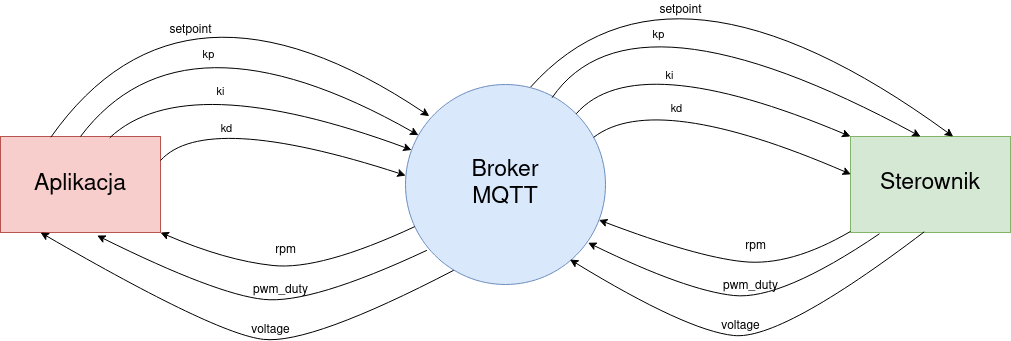
\includegraphics[width=1\textwidth]{img/dane.png}
      \caption{Schemat wymiany danych w systemie}
      \label{data_transmision}
    \end{figure}